%==============================================================================
% Sjabloon onderzoeksvoorstel bachelorproef
%==============================================================================
% Gebaseerd op LaTeX-sjabloon ‘Stylish Article’ (zie voorstel.cls)
% Auteur: Jens Buysse, Bert Van Vreckem
%
% Compileren in TeXstudio:
%
% - Zorg dat Biber de bibliografie compileert (en niet Biblatex)
%   Options > Configure > Build > Default Bibliography Tool: "txs:///biber"
% - F5 om te compileren en het resultaat te bekijken.
% - Als de bibliografie niet zichtbaar is, probeer dan F5 - F8 - F5
%   Met F8 compileer je de bibliografie apart.
%
% Als je JabRef gebruikt voor het bijhouden van de bibliografie, zorg dan
% dat je in ``biblatex''-modus opslaat: File > Switch to BibLaTeX mode.

\documentclass{voorstel}
\usepackage{pgfplots}
\usepackage{lipsum}
%\usepackage{geometry}\right) 
\pgfplotsset{compat=newest}
%\geometry{left=0mm, right=3mm,top=6mm, bottom=3mm,}
\definecolor{mygr}{HTML}{e6e6e6}

%------------------------------------------------------------------------------
% Metadata over het voorstel
%------------------------------------------------------------------------------

%---------- Titel & auteur ----------------------------------------------------

% TODO: geef werktitel van je eigen voorstel op
\PaperTitle{Hoe kunnen we een evoluerend bedrijfsnetwerk beter beveiligen door het gebruik van Cisco ISE?}
\PaperType{Onderzoeksvoorstel Bachelorproef 2019-2020} % Type document

% TODO: vul je eigen naam in als auteur, geef ook je emailadres mee!
\Authors{Joeri Verhavert\textsuperscript{1}} % Authors
\CoPromotor{Dean De Blieck\textsuperscript{2} (Fit It - Axians)}
\affiliation{\textbf{Contact:}
  \textsuperscript{1} \href{mailto:joeri.verhavert.y7236@student.hogent.be}{joeri.verhavert.y7236@student.hogent.be};
  \textsuperscript{2} \href{mailto:dean.deblieck@axians.com}{dean.deblieck@axians.com};
}

%---------- Abstract ----------------------------------------------------------

\Abstract{
Naarmate Internet of Things en Bring Your Own Device blijven uitbreiden, wordt het potentieel cyber aanvalspercentage steeds groter op ondernemingsvlak. Nieuwe zwakheden en kwetsbaarheden in het networkdomein worden steeds opnieuw blootgelegd. Met als gevolg hebben bedrijven een verbeterde toegangscontrole nodig om endpoint apparaten en het netwerk beter te beschermen tegen interne en externe threads. De integratie van Cisco Identity Service Engine in het bedrijfsnetwerk kan hierbij een oplossing zijn voor deze problematiek. Cisco Identity Service Engine biedt een netwerk gebaseerde aanpak voor een aanpasbare en vertrouwde toegang van overal. Door deze integratie verwacht men enerzijds een beter beheer in endpoint-systemen door monitoring, etc... en anderzijds verwacht men een betere beveiliging van de grote toename in systemen die connectie maken met het netwerk door Policy Based Access Control, Network Access Control, etc... Er zijn vele uitbreidingen/Use cases denkbaar die hiervoor een oplossing kunnen bieden, maar de belangrijkste use cases die toegepast zullen worden tijdens de bachelorproef zijn: toegang op het netwerk met Policy Based Access Control, Threat-centric Network Access Control en Port Based Access Control.

%--	Hier schrijf je de samenvatting van je voorstel, als een doorlopende tekst van één paragraaf. Wat hier zeker in moet vermeld worden: \textbf{Context} (Waarom is %--dit werk belangrijk?); \textbf{Nood} (Waarom moet dit onderzocht worden?); \textbf{Taak} (Wat ga je (ongeveer) doen?); \textbf{Object} (Wat staat in dit document %--geschreven?); \textbf{Resultaat} (Wat verwacht je van je onderzoek?); \textbf{Conclusie} (Wat verwacht je van van de conclusies?); \textbf{Perspectief} (Wat zegt de %--toekomst voor dit werk?).
%--Bij de sleutelwoorden geef je het onderzoeksdomein, samen met andere sleutelwoorden die je werk beschrijven.
%--Vergeet ook niet je co-promotor op te geven.
}

%---------- Onderzoeksdomein en sleutelwoorden --------------------------------
% TODO: Sleutelwoorden:
%
% Het eerste sleutelwoord beschrijft het onderzoeksdomein. Je kan kiezen uit
% deze lijst:
%
% - Mobiele applicatieontwikkeling
% - Webapplicatieontwikkeling
% - Applicatieontwikkeling (andere)
% - Systeembeheer
% - Netwerkbeheer
% - Mainframe
% - E-business
% - Databanken en big data
% - Machineleertechnieken en kunstmatige intelligentie
% - Andere (specifieer)
%
% De andere sleutelwoorden zijn vrij te kiezen

\Keywords{Netwerkbeheer, NAC, ISE, PDAC, Cybersecurity, Cisco} % Keywords
\newcommand{\keywordname}{Sleutelwoorden} % Defines the keywords heading name

%---------- Titel, inhoud -----------------------------------------------------

\begin{document}

\flushbottom % Makes all text pages the same height
\maketitle % Print the title and abstract box
\tableofcontents % Print the contents section
\thispagestyle{empty} % Removes page numbering from the first page

%------------------------------------------------------------------------------
% Hoofdtekst
%------------------------------------------------------------------------------

% De hoofdtekst van het voorstel zit in een apart bestand, zodat het makkelijk
% kan opgenomen worden in de bijlagen van de bachelorproef zelf.
%---------- Inleiding ------------s---------------------------------------------

\section{Introductie} % The \section*{} command stops section numbering
\label{sec:introductie}
Tijdens deze uiteenzetting zal voornamelijk beschreven worden hoe Network Access Control door het gebruik van de technologie Cisco Identity Service Engine (\cite{CiscoISE}) gebruikt wordt.\\Door principes zoals Bring Your Own Device (BYOD) en Internet Of Things (IoT) is er steeds meer vraag naar de bussiness resources van de verschillende endpoint-systemen vanuit het perspectief van de werknemers of de IoT-systemen. Bedrijven moeten de proliferatie netwerk-compatibele apparaten beter ondersteunen, zelfs wanneer een groot aantal cyber bedreigingen en veel gepubliceerde datalekken aantonen dat het belang van bescherming over de toegang tot de ontwikkelende bedrijfsnetwerken van cruciaal belang is.\\Door integratie van Cisco Identity Service Engine kan er een betere bescherming gegarandeerd worden tegen deze exponentiële toename van geconnecteerde systemen. Kortom kan het netwerk veiliger en meer beheerbaar gemaakt worden. Uit deze informatie kan een antwoord op de volgende onderzoeksvragen een oplossing bieden in dit probleemveld. De onderzoeksvragen luiden als volgt: Hoe kunnen we een evoluerend bedrijfsnetwerk beter beheren en beveiligen door het gebruik van Cisco Identity Service Engine? Hoe zorgen we voor een veiliger IT netwerk met principes zoals Internet Of Things en Bring Your Own Device? Wat zijn de positieve en negatieve gevolgen door het gebruik van Cisco Identity Service Engine?\\ \\Cisco Identity Service Engine is een groot platform waar vele uitbreidingen en use cases mogelijk zijn, daarom zal Policy Based Access Control, Threat-centric Network Access Control en Port-based Network Access Control als basis toegepast worden tijdens de uiteenzetting van deze bachelorproef.

%---------- Stand van zaken ---------------------------------------------------
\pagebreak
\section{Literatuurstudie}
\label{sec:Literatuurstudie}
U vraagt zich waarschijnlijk af wat termen zoals Network Access Control, Policy Based Access Control, Threat-centric Network Access Control en Port Based Network Access Control nu eigenlijk betekenen?\\Volgens \cite{Cisco} is Network Access Control, een oplossingen die netwerkzichtbaarheid en toegangsbeheer ondersteunt door middel van beleidshandhaving op apparaten en gebruikers in bedrijfsnetwerken. Organisaties moeten rekening houden met de veiligheidsrisico's van de exponentiële groei van verscheidene endpoint-systemen die toegang hebben op het bedrijfsnetwerk. Cisco beweert dat het van cruciaal belang is om over de correcte tools te beschikken die het netwerkbeveiligings infrastructuur versterken.

\subsection{Network Access Control use cases}
Zaken zoals Policy Based Access Control, Threat-centric Network Access Control en Port Based Network Access Control zijn termen die gezien worden als use cases of als uitbreiding van de Network Access Control technologie. Deze use cases hebben allemaal als functie het netwerk veilig te maken tegen interne of externe threads. Zo zorgt volgens \cite{jerichosystems.net} Policy Based Access Control voor een beter digitaal beheer dat bestaat uit verschillende regels om beslissingen te nemen op de authorization levels. \\\cite{TC-NAC} citeert dat Threat-centric Network Access Control zich ontfermt over het creëren van policies die gebaseerd zijn 
op de bedreigings- en kwetsbaarheidskenmerken die komen vanuit endpoint systemen. Als laatste term hebben we Port Based Network Access Control,\\\cite{juniper.net} vertelt ons dat Port Based Network Access Control, Ethernet-interfaces valideert om ongeautoriseerde toegang tot een opgegeven routerpoort te voorkomen. Voordat deze authenticatie voltooid is, zijn alleen de 802.1x-besturingspakketten toegestaan en worden deze doorgestuurd naar de router voor verwerking. De overige besturingspakketten worden verwijderd.


\subsection{Award uitreiking}
De award uitreiking die Frost and Sullivan heeft uitgevoerd over Cisco Identity Service Engine wordt tijdens deze sectie aangehaald. Gebaseerd op recente analyses en onderzoeken van wereldwijde Network Access Controls, erkent \cite{Frost&Sullivan} Cisco Systems met de Global Market Leadership Award voor het veroveren van ongeveer 35 percent van de markt. Dit heeft vooral te maken met Cisco's brede portfolio van beveiligingsproducten. Volgens Frost en Sullivan heeft Cisco Identity Services Engine de grote bedrijfssegmenten volledig gedomineerd. De integratie van Cisco Identity Service Engine brengt veel uitgebreide en schaalbare oplossingen met zich mee, die een breed gamma aan functies hebben. \\ \\ Cisco won de uitreiking van de Global Market Leadership Award mede dankzij de recente release van de Identity Service Engine 2.4. De release van 2.4 breidt zijn talrijke functies uit naar opkomende industriële markten, zoals Internet of Things, de industrie- en de gezondheidszorgmarkt. Cisco werkt hiervoor samen met ziekenhuizen, fabrieken, etc.. , om een oplossing te ontwikkelen die niet enkel medische systemen identificeert, maar ook helpt bij het definiëren van het toegangsniveau's van systemen op het netwerk.
%--Hier beschrijf je de \emph{state-of-the-art} rondom je gekozen onderzoeksdomein. Dit kan bijvoorbeeld een literatuurstudie zijn. Je mag de titel van deze sectie ook %--aanpassen (literatuurstudie, stand van zaken, enz.). Zijn er al gelijkaardige onderzoeken gevoerd? Wat concluderen ze? Wat is het verschil met jouw onderzoek? Wat %--is de relevantie met jouw onderzoek?

%--Verwijs bij elke introductie van een term of bewering over het domein naar de vakliteratuur, bijvoorbeeld~\autocite{Doll1954}! Denk zeker goed na welke werken je %--refereert en waarom.

% Voor literatuurverwijzingen zijn er twee belangrijke commando's:
% \autocite{KEY} => (Auteur, jaartal) Gebruik dit als de naam van de auteur
%   geen onderdeel is van de zin.
% \textcite{KEY} => Auteur (jaartal)  Gebruik dit als de auteursnaam wel een
%   functie heeft in de zin (bv. ``Uit onderzoek door Doll & Hill (1954) bleek
%   ...'')

%--Je mag gerust gebruik maken van subsecties in dit onderdeel.

%---------- Methodologie ------------------------------------------------------
\section{Methodologie}
\label{sec:methodologie}
Om het onderzoek tot een goed einde te brengen, zullen onderzoekstechnieken zoals experimenten, simulaties, implementatie en eventuele enquêtes worden toegepast tijdens dit onderzoek. Axians zal hiervoor een testomgeving voorzien waar Cisco Identity Service Engine uitgerold kan worden. Deze uitvoering zal samen met Policy Based Access Control en threat-Centric Network Access Control geïmplementeerd worden. Indien de tijd dit toelaat, is er een mogelijkheid om extra Use cases te gaan implementeren in de testomgeving om het onderzoek naar een beter beheerbaar en veiliger groeiend bedrijfsnetwerk uit te breiden. Daarnaast zullen er een aantal experimenten en simulaties uitgevoerd worden. Dit laat het toe om acties van uit de werkelijkheid na te bootsen in de voorziene testomgeving. Een mogelijk voorbeeld van experiment kan zijn dat men door de integratie van Threat-Centric Network Access Control het mogelijk maakt dat een geïnfecteerd endpoint-systeem automatisch "weg geknipt" 
wordt uit het bedrijfsnetwerk. Deze actie voorkomt dus dat andere endpoint-systemen ook geïnfecteert zullen raken.\\ \\Om het onderzoek verder aan te vullen, kunnen er enquêtes worden opgesteld. Op deze manier kan in kaart gebracht worden waarom, Axians Cisco Identity Service Engine verkiest boven een andere NAC technologie, welke positieve en negatieve punten Axians ondervindt bij het gebruik van Cisco Identity Service Engine, of indien Axians een daling van interne of externe threads ondervindt sinds de implementatie van Cisco Identity Service Engine.
%--Hier beschrijf je hoe je van plan bent het onderzoek te voeren. Welke onderzoekstechniek ga je toepassen om elk van je onderzoeksvragen te beantwoorden? Gebruik je %--hiervoor experimenten, vragenlijsten, simulaties? Je beschrijft ook al welke tools je denkt hiervoor te gebruiken of te ontwikkelen.


%---------- Verwachte resultaten ----------------------------------------------
\section{Verwachte resultaten}
\label{sec:verwachte_resultaten}
%De bedoeling van deze sectie is om de verwachten resultaten op te stellen over een aantal variabelen die we wensen te testen.
De bedoeling van deze sectie is om stil te staan over de verwachte resultaten van het onderzoek. Op het einde van het onderzoek moet het belang van een Network Access Control aangetoond worden. Eveneens wordt een zeer snelle handeling verwacht tijdens een ramp scenario door het gebruik van Threat-Centric Network Access Control. Dit kan aangetoond worden door het uitvoeren van talrijke experimenten die acties uit de werkelijkheid nabootsen. Daarom wordt de nadruk zeer hard gelegd op een zo goed mogelijke implementatie. Enkel op deze manier kan er aangetoond worden dat de implementatie hierbij leidt tot een veiliger, beheerbaar netwerk. Er wordt verwacht dat de kans op succesvolle cyberaanvallen door de interne en externe threads aanzienlijk kleiner zal zijn door het gebruik van Cisco Identity Service Engine. Dit kunnen we perfect aantonen door gebruik te maken van een mockgrafiek. Door het gebruik van mockgrafieken wordt er een beter visueel beeld gecreëerd van de resultaten.
%\begin{wrapfigure}{2}{0.15\textwidth}
%	\centering
%	\includegraphics[height=0.55\textwidth,height=.35\textheight]{images/KansRampSenarios.jpg}
%\end{wrapfigure}
\\ \\
\begin{figure}[!t]
	\centering
	\textbf{Kans op succesvolle cyberaanvallen}\par\medskip
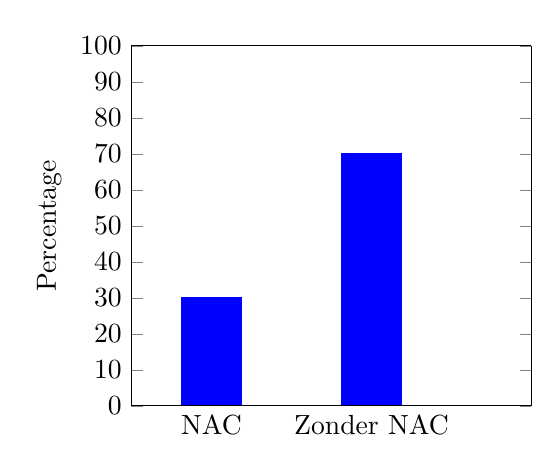
\begin{tikzpicture}
\begin{axis}[
	/pgf/number format/1000 sep={},
	width=2.0in,
	height=1.8in,
	at={(0.758in,3in)},
	scale only axis,
	clip=false,
	separate axis lines,
	axis on top,
	xmin=0,
	xmax=5,
	xtick={1,2,3},
	x tick style={draw=none},
	xticklabels={NAC, ,Zonder NAC},
	ytick={0,10,20,30,40,50,60,70,80,90,100},
	ymin=0,
	ymax=100,
	ylabel={Percentage},
	every axis plot/.append style={
		ybar,
		bar width=0.3in,
		bar shift=0pt,
		fill
	}
	]
	\addplot[blue]coordinates{(1,30)};
	\addplot[blue]coordinates{(3,70)};
\end{axis}
\end{tikzpicture}
\end{figure}

%---------- Verwachte conclusies ----------------------------------------------
\section{Verwachte conclusies}
\label{sec:verwachte_conclusies}
Wanneer de resultaten van het onderzoek aanduiden dat bedrijven die NAC technologieën implementeren, hun endpoint systemen beter kunnen beheren en beveiligen tegen interne en externe threads. Dan kunnen we concluderen dat het belang van deze implementaties rondom de Network Access Control technologieën een belangrijke must is. Daarnaast verwachten we ook dat het percentage op cyberaanvallen op het netwerk aanzienlijk kleiner zal zijn. Bovendien verwachten we dat met het gebruik van Network Access Control in combinatie met Threat-centric Network Access Control een zeer snelle handeling gebeurt wannneer endpoint systemen virussen of malware bevat.

%--Hier beschrijf je wat je verwacht uit je onderzoek, met de motivatie waarom. Het is \textbf{niet} erg indien uit je onderzoek andere resultaten en conclusies vloeien dan dat je hier beschrijft: het is dan juist interessant om te onderzoeken waarom jouw hypothesen niet overeenkomen met de resultaten.



%------------------------------------------------------------------------------
% Referentielijst
%------------------------------------------------------------------------------
% TODO: de gerefereerde werken moeten in BibTeX-bestand ``voorstel.bib''
% voorkomen. Gebruik JabRef om je bibliografie bij te houden en vergeet niet
% om compatibiliteit met Biber/BibLaTeX aan te zetten (File > Switch to
% BibLaTeX mode)

\phantomsection
\printbibliography[heading=bibintoc]

\end{document}
